\chapter{Applications}
\label{ch:Applications}
\section{Introduction}

The data-sets were split into a training and a test set. The training data consists of \nicefrac{3}{4}'th of the data while the test set contains the other \nicefrac{1}{4}'th.\\

\section{Implementations and tuning parameters of the methods}
\label{sec:implementation}
For the majority of the methods described in Chapters \ref{ch:ReducingTheNumberOfExplanatoryVariables} and \ref{ch:ClassificationTechniques} some decisions regarding their model specification and tuning parameters have to be made.

In order to have a nice baseline method the logistic model was fit by using only linear terms. The logistic regression methods combined with the lasso or ridge were fit by using a cubic polynomial expansion of the predictors. To limit the amount of predictors and computational cost no interaction terms were considered. \\

It was decided to implement our own version of PCA logistic and KPCA logistic regression. This was mainly done to investigate the remarks made in Section \ref{sec:dimRedPrVSBG}. Both implementations allow us to specify on which indices the (K)PCA should be based on. Furthermore 5-fold-CV is used to select the an optimal number of principal components where always the components corresponding to the $x$ highest eigenvalues. To allow some non-linearity in the PCA logistic regressin implementation we also allow for polynomial expansions in the PCs of up to the third degree (ignoring interaction effects). CV is used to select the optimal polynomial expansion. This expanding of the PCs into a polynomial is not done when KPCA is used, the reason is that KPCA already implicitly expands the original data into a new non-linear expansion. To limit the computational costs it was decided to limit the number of components to at most $75$ in the KPCA implementation. Furthermore, when using KPCA together with logistic regression the KPCA will be performed on at most $500$ observations, if necessary these are randomly selected from the relevant observations. \\

In the MaxEnt implementation where CV was used to select the regularization parameters considered were $\chi \times \lambda_{def}$ with $\lambda_{def}$ the default MaxEnt parameter and $\chi \in \{0.1,0.5,1,2,10\}$. \\

The tuning variables and of the ANN method are the number of neurons and the in the hidden layer $\in \{ 5,10,20,40,60 \}$. Following the suggestions of \cite{venables_modern_2002} we optimize the weight decay parameter over $\{0.1,0.01,0.001,0.0001\}$. Furthermore instead of simply averaging neural networks it was decided to use bagging which has, next to the advantages mentioned in Section \ref{sec:ANN}, the advantage that it tends to prevent over-fitting. The only tuning parameter that is used in the vanilla ANN model is the number of neurons in the hidden layer. \\

The tuning parameters of our gradient boosted decision trees are the number of trees $\in \{ 100,500,1000,2000\}$, the interaction depth $\in \{ 1,3,5,7\}$, and the amount of shrinkage $\in  \{0.1,0.01,0.001,0.0001)\}$. The choice of these values was mainly inspired by \cite{elith_working_2008}. \\

\section{AUC as a measure of classification performance in SDM}
\label{sec:AUC}
To measure the performance of the classification method the area under the receiver operating curve (AUC) values will be used. Using the AUC to measure the performance of SDMs has been criticized \parencite{lobo_auc:_2008, jimenez-valverde_insights_2012}. However, most of the issues that are usually raised are not of particular interest in our case. Before studying the AUC values it is interesting to note that there are three main sources of randomness in the calculation of the mean AUC values across the different species. \\ 

First of all, in our set-up we could consider the species that are considered as drawn from a pool of all species in the databases. Of course this assumption is violated since we selected the species conditional on certain characteristics.  \\

Secondly, the parameters in the classifications methods are estimated by using the training set. The elements of the training set can be seen sample of presence, and background or absence points from the corresponding distributions. The predicted variables, and the AUC, are therefore also dependent on the sample of points used. \\

Thirdly, the AUC is calculated on the test set which again consists of a sample of random presence, and background or absence points from the corresponding distributions. Thus even if the classifier was fixed we would get different AUC values if we use different test sets. \\

It is well known that the AUC statistic is equivalent to the Mann-Whitney U test statistic \parencite{hanley_meaning_1982} and hence the theory surrounding the Mann-Whitney U test statistic can provide us with standard errors (SE), asymptotic distributions, etc. However, these results only hold if the classifier is assumed to be fixed and hence ignores the randomness of the methods themselves and the species sampling scheme. A rigorous way to inspect the distribution of the AUC values would be to use a bootstrap method to construct e.g.\ confidence intervals. In our situation this is however computationally infeasible. In the end we opted to only report standard deviations (SD) and the mean values.\\

\section{Presence-only data}

\subsection{Results}
All the methods described in Sections \ref{sec:combinations} and \ref{sec:implementation} were fitted upon the GBIF data. Summary measures of the AUC values can be found in Table \ref{tab:PrOnlyAUC} and Figure \ref{fig:PrOnlyAUC}.


\begin{table}[!htb]
\makebox[\textwidth][c]{
\begin{tabular}{lcccccc}
 & \multicolumn{2}{c}{All variables} & \multicolumn{2}{c}{Bioclimatic variables} & \multicolumn{2}{c}{Difference}\\
\cline{2-3} \cline{4-5} \cline{6-7}\\
Method & Mean AUC & SD & Mean AUC & SD & Mean AUC & SD \\
\midrule
Logistic: vanilla               & 0.934 & 0.045 & 0.916 & 0.070 & 0.019    & 0.053 \\
Logistic: backward              & 0.772 & 0.266 & 0.934 & 0.035 & -0.162   & 0.262 \\
Logistic: forward               & 0.661 & 0.242 & 0.599 & 0.277 & 0.062    & 0.330 \\
Logistic: PCA                   & 0.891 & 0.077 & 0.881 & 0.087 & 0.010    & 0.070 \\
Logistic: presence PCA          & 0.838 & 0.172 & 0.887 & 0.090 & -0.049   & 0.101 \\
Logistic: background PCA        & 0.893 & 0.079 & 0.890 & 0.077 & 0.003    & 0.054 \\
Logistic: kernel PCA            & 0.933 & 0.050 & 0.922 & 0.058 & 0.011    & 0.030 \\
Logistic: presence kernel PCA   & 0.947 & 0.033 & 0.927 & 0.052 & 0.020    & 0.040 \\
Logistic: background kernel PCA & 0.937 & 0.048 & 0.935 & 0.039 & 0.002    & 0.028 \\
Logistic: lasso                 & 0.938 & 0.041 & 0.924 & 0.057 & 0.014    & 0.037 \\
Logistic: ridge                 & 0.930 & 0.047 & 0.908 & 0.063 & 0.022    & 0.039 \\
Logistic: select07              & 0.938 & 0.040 & 0.915 & 0.058 & 0.023    & 0.032 \\
GAM: auto selection             & 0.928 & 0.072 & 0.935 & 0.033 & -0.008   & 0.069 \\
GAM: vanilla                    & 0.912 & 0.086 & 0.936 & 0.038 & -0.024   & 0.090 \\
GAM: select07                   & 0.940 & 0.050 & 0.938 & 0.036 & 0.002    & 0.039 \\
MaxEnt                          & 0.921 & 0.055 & 0.932 & 0.041 & -0.011   & 0.028 \\
MaxEnt Vanilla                  & 0.899 & 0.099 & 0.919 & 0.049 & -0.020   & 0.076 \\
ANN                             & 0.946 & 0.046 & 0.948 & 0.032 & -0.003   & 0.040 \\
ANN: vanilla                    & 0.926 & 0.058 & 0.934 & 0.039 & -0.008   & 0.048 \\
GBM                             & 0.958 & 0.032 & 0.944 & 0.033 & 0.014    & 0.030 \\
\bottomrule
\end{tabular}}
\caption{\label{tab:PrOnlyAUC}Summary of the AUC values of the different classifiers fitted on the presence-only data.}
\end{table}

\begin{figure}[!htb]
\center
\makebox[\textwidth][c]{%
	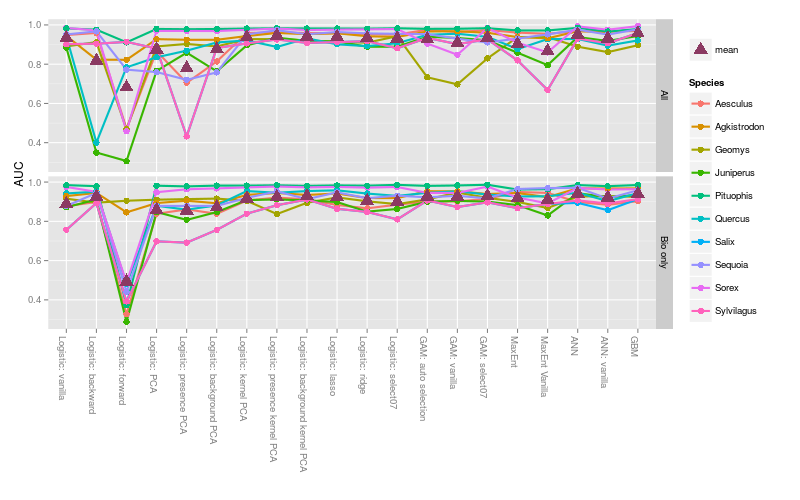
\includegraphics[scale=0.70]{Plots/AUCPlot.png}
}
\caption{\label{fig:PrOnlyAUC}AUC values of the different classifiers fitted on the presence-only data.}
\end{figure}

First of all, few rigorous tests will be performed in this section. This because given the small sample size and the fact that the AUC values are quite close the power of such tests, using the usual $5\%$ significance level, is very low. Because of this the discussion is rather short and mainly used as a preliminary study which generated interesting research questions for the simulation study of Chapter \ref{chap:SimulationStudy}. \\

It is interesting to note that logistic regression performs quite well. Furthermore, the SDs of the stepwise selection methods are relatively large. This might indicate that these methods are inherently variable and hence lead to unstable predictions. It is interesting to note that while the performance of forward stepwise selection is bad when all variables are considered this is not the case when only the bioclimatic variables are considered. This could be explained by the fact that the backward selection method becomes a lot more variable when variables with little explanatory power are added. However, since this is a variable selection technique this is unwanted behaviour. The MaxEnt implementation that uses the default settings performs worse than the implementation in which the penalization parameter is selected by CV. Perhaps the most interesting is that GBM and ANNs seem to consistently lead to high AUC values with low standard deviations. Given our results it seems like MaxEnt might be overused throughout the standard deviations and at least some other machine learning methods should at least be considered before opting for MaxEnt. \\

In light of the discussion in Section \ref{sec:dimRedPrVSBG} two Wilcoxon signed-rank tests were performed to test whether there is a significant difference between performing the (K)PCA on the background points or on the presence points. The p-value corresponding with the test for the PCA (resp.\ KPCA) is $0.32$ (resp.\ $0.11$) and hence accept the null-hypothesis of no difference between the methods.

To test whether or not using only the bioclimatic variables has a profound effect a Wilcoxon signed-rank test was performed for each method. These tests are of interest because on one hand they provide information on the usefulness of non-bioclimatic variables, i.e. is there an increase in classification performance. Also the a decrease in classification performance is of interest to detect, this could be interpreted as adding irrelevant predictors which lead to over-fitting. Even before performing a multiple testing correction none of the tests were significant at the $5$\% level. Hence we conclude that in our limited study there's no difference between using only the bioclimatic variables or all variables. 

\section{Presence-absence data}
Although a variation of the MaxEnt method can be used for presence-only data this is nearly never done. Furthermore, instead of fitting three different variations of (K)PCA logistic regression it was decided to only use the standard approach. This was done to speed up the computations, and unlike what was he case in the presence-only scenario the absence points are ``real'' observations. Since only five species were considered there are no statistically significant results in this section. The inspection is mainly done to make sure that the different methods show approximately have the same performance characteristics for both presence-only and presence-absence data. The results can be found in Section \ref{sec:PAResults}. Finally, because there are at between $42029$ and $287860$ plot locations available the fitting of the models leads to computational problems. A solution to these problems is proposed in Section \ref{sec:CaseControlSubsampling}
\subsection{Case-control sampling}
\label{sec:CaseControlSubsampling}
Because of computational considerations it was decided to use a subset of the presence-absence data to fit the models upon. More particularly, the subsample consists of all the presence points and $5000$ randomly sampled absence points. This is clearly a form of case-control sampling and the effect of doing this has been studied to some extent \parencite{king_logistic_2001}. \\

In the case of logistic regression some algebra along the lines of Equation \ref{eq:IPPSampling} shows that only the intercept is affected by the sub-sampling \parencite{king_logistic_2001}. Although the underlying coefficients stay the same the variance of the estimators should increase slightly. Because we only subsample the absence points this increase should be somewhat limited. Intuitively it makes sense that a rare presence point contains more information about the coefficients than one of the abundant absence points. In the case of logistic regression this can rigorously be deduced by observing that a term of the form $P(Y=1|\bm{X} = \bm{x}) \left[1- P(Y=1|\bm{X} = \bm{x}) \right]$ turns up in the variance expression. Usually this term is quite a lot smaller for the abundant cases and hence leaving some out does not lead to a huge increase of the variance. \\ 

Although the previous paragraph focusses on logistic regression the same reasoning can be applied to the other methods considered. Finally, in the last two decades there has been quite some research on imbalanced data-sets and perhaps more efficient ways of dealing with the imbalance exist, see e.g.\ \cite{chawla2005data} for an overview of other methods. \\

\subsection{results}
\label{sec:sec:PAResults}
The mean and and the standard deviations can be found in Table \ref{tab:PrAbAUC} and Figure \ref{fig:PrAbAUC} shows a plot of the estimated AUC values. \\

\begin{table}[!htb]
\makebox[\textwidth][c]{
\begin{tabular}{lcccccc}
 & \multicolumn{2}{c}{All variables} & \multicolumn{2}{c}{Bioclimatic variables} & \multicolumn{2}{c}{Difference}\\
\cline{2-3} \cline{4-5} \cline{6-7}\\
Method & Mean AUC & SD & Mean AUC & SD & Mean AUC & SD \\
\midrule
Logistic: vanilla    & 0.961 & 0.027 & 0.960 & 0.028 & 0.001  & 0.001 \\
Logistic: backward   & 0.682 & 0.301 & 0.656 & 0.318 & 0.026  & 0.345 \\
Logistic: forward    & 0.774 & 0.284 & 0.741 & 0.256 & 0.034  & 0.046 \\
Logistic: PCA        & 0.913 & 0.084 & 0.913 & 0.084 & 0.000  & 0.000 \\
Logistic: kernel PCA & 0.950 & 0.052 & 0.950 & 0.052 & 0.000  & 0.000 \\
Logistic: lasso      & 0.960 & 0.042 & 0.960 & 0.042 & 0.000  & 0.000 \\
Logistic: ridge      & 0.957 & 0.044 & 0.957 & 0.044 & 0.000  & 0.000 \\
Logistic: select07   & 0.756 & 0.239 & 0.756 & 0.239 & 0.000  & 0.000 \\
GAM: auto selection  & 0.925 & 0.098 & 0.925 & 0.098 & 0.000  & 0.000 \\
GAM: vanilla         & 0.877 & 0.117 & 0.877 & 0.117 & 0.000  & 0.000 \\
GAM: select07        & 0.948 & 0.062 & 0.948 & 0.062 & 0.000  & 0.000 \\
ANN                  & 0.973 & 0.020 & 0.972 & 0.021 & 0.001  & 0.002 \\
ANN: vanilla         & 0.962 & 0.036 & 0.969 & 0.029 & -0.007 & 0.014 \\
GBM                  & 0.977 & 0.014 & 0.977 & 0.014 & 0.000  & 0.000 \\
\bottomrule
\end{tabular}}
\caption{\label{tab:PrAbAUC}Summary of the AUC values of the different classifiers fitted on the presence-absence data.}
\end{table}


\begin{figure}[!htb]
\center
\makebox[\textwidth][c]{%
	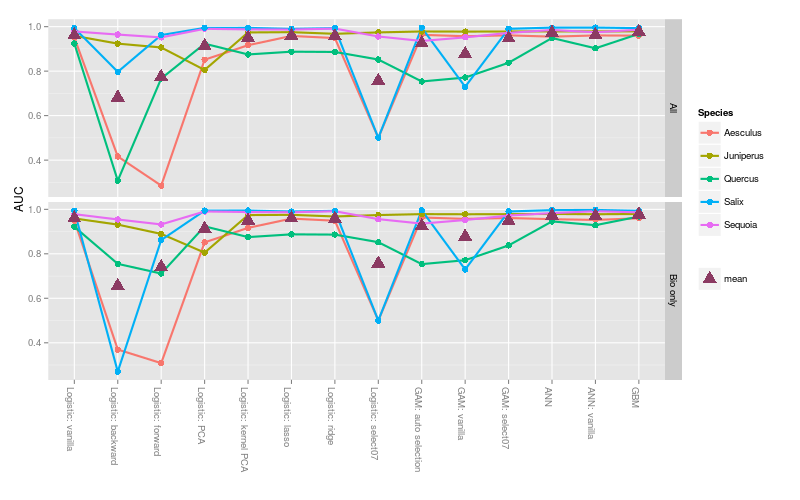
\includegraphics[scale=0.70]{Plots/AUCPAPlot.png}
}
\caption{\label{fig:PrAbAUC}AUC values of the different classifiers fitted on the presence-absence data.}
\end{figure}

It is readily seen that the logistic regression model performs quite well, i.e. it leads to relatively high average AUC values and its SD is quite low. The stepwise methods both have large SD and have the lowest average AUC values. The GBM and ANN methods are the two methods with the largest average AUC and both have relatively small SD. Unlike in the presence-only scenario the logistic07 methods has quite a large variance and performs quite badly. Finally, the differences between using the bioclimatic or all variables are extremely small, 



\section{Discussion}

